%%%%%%%%%%%%%%%%%%%%%%%%%%%%%%%%%%%%%%%%%%%%%%%%%%%%%%%%%%%%%%%%%%%%%%%%%%%%%%
% ASU Dissertation Quarto Template
%%%%%%%%%%%%%%%%%%%%%%%%%%%%%%%%%%%%%%%%%%%%%%%%%%%%%%%%%%%%%%%%%%%%%%%%%%%%%%
% Revised by Julian Tao based on Robert W. Kutter's version
%
% For guidance on using this file, see the README.
%
%%%%%%%%%%%%%%%%%%%%%%%%%%%%%%%%%%%%%%%%%%%%%%%%%%%%%%%%%%%%%%%%%%%%%%%%%%%%%%
% Preamble
%%%%%%%%%%%%%%%%%%%%%%%%%%%%%%%%%%%%%%%%%%%%%%%%%%%%%%%%%%%%%%%%%%%%%%%%%%%%%%
\newcommand*{\pointsize}{12pt}          %<Set the font size; make sure the size is correct
                                        %   for the font you will use
\documentclass[letterpaper,             % Use US letter-size paper
               oneside,                 % No verso and recto differences
               \pointsize]              % Uses the font size defined above
               {memoir}
\renewcommand{\cleardoublepage}%        % \cleardoublepage will create entirely blank
  {\clearpage}%                         %   pages depending on settings (e.g., usually
                                        %   before start of \mainmatter); redefine it here
                                        %   so that no entirely blank pages are created
                                        %   automatically
%%%%%%%%%%%%%%%%%%%%%%%%%%%%%%%%%%%%%%%
% (Some) Packages
%%%%%%%%%%%%%%%%%%%%%%%%%%%%%%%%%%%%%%%
\usepackage{newtxtext,newtxmath}        % Times New Roman
\usepackage{graphicx}                   % For importing image files
\usepackage{etoolbox}                   % For advanced commands throughout preamble
\usepackage[dvipsnames]{xcolor}
\usepackage{microtype}                  %~Improves kerning and protrusion (optional);
                                        %   See here for an introduction:
                                        %   http://www.khirevich.com/latex/microtype/

\providetoggle{usemicrotype}            % TRUE = microtype is being used
\makeatletter                           %   (Used to turn of microtype protrusion in the
\@ifpackageloaded{microtype}%           %   table of contents.)
  {\settoggle{usemicrotype}{true}}%
  {\settoggle{usemicrotype}{false}}
\makeatother
\usepackage{changepage}                 % For changing page layout (e.g., margins) in the
                                        %   middle of the document
\usepackage{calc}					              % Calculate text widths; used in page layout
                                        %   changes

%%%%%%%%%%%%%%%%%%%%%%%%%%%%%%%%%%%%%%%
% Title page, input
%%%%%%%%%%%%%%%%%%%%%%%%%%%%%%%%%%%%%%%

\listadd{\titlelines}{A Thesis Submitted for a PhD degree at
ASU}             

\newcommand*\Author{John
Doe}          %<Enter your name; must match official transcript
\newcommand*{\documentname}%
  {Dissertation}                        %<Enter the type of document (capitalized)
\newcommand*{\degreename}
  {Doctor of
Philosophy}                %<Enter the type of degree (capitalized)
\newcommand*\defdate{July
2023}        %<Give month (written out fully) and year of
                                        %   the oral defense
\listadd{\committeechair}{Jane
Smith}   %<Enter committee chair name; use \listadd for
%\listadd{\committeechair}{Another name}%   for additional names
\newcommand*{\chairlabel}{Chair(s)}        %<If you have co-chairs, replace this text with
                                        %   'Co-Chair'
\listadd{\committeemember}{Joe
Bloggs} %<Enter committee member names; use \listadd for
\listadd{\committeemember}{So-and-so} %<Enter committee member names; use \listadd for
\newcommand*{\gradmonth}{May}           %<Enter the graduation date; month can only be:
                                        %  May, August, or December
\newcommand*{\gradyear}{2023}           %<Enter the graduation year, e.g. 2014

\listadd{\keywords}{lorem}          %<Enter keywords; use \listadd for
\listadd{\keywords}{ipsum}          %<Enter keywords; use \listadd for
\newcommand*{\graddate}{\gradmonth%     % Compose full graduation date
  \space\gradyear}

%%%%%%%%%%%%%%%%%%%%%%%%%%%%%%%%%%%%%%%
% Page layout
%%%%%%%%%%%%%%%%%%%%%%%%%%%%%%%%%%%%%%%
\settrimmedsize{\stockheight}%          % Specifies \paperheight and \paperwidth
  {\stockwidth}{*}
\settrims{0pt}{0pt}                     % Set location of page in relation to the stock.
                                        % Paper and stock size are equivalent,
                                        % so both \trimtop and \trimedge are set to 0pt
\newlength{\forfootskip}
\setlength{\forfootskip}%
  {3\baselineskip}
\newlength{\textblockheight}            % Calculate height of text block to leave room
\setlength{\textblockheight}{9.0in}     %   for footers, keeping page numbers outside
\addtolength{\textblockheight}%         %   the 1in vertical margins
  {-\forfootskip}
\settypeblocksize{\textblockheight}%    % Calculated by 1.0in vertical margins and
  {*}{*}                                %   letting margins set the width of the typeblock
\setulmargins{1.0in}{*}{*}              % Set upper margin (\uppermargin, not \topmargin);
                                        %   calculate the bottom margin
\setlrmarginsandblock{1.25in}{1.25in}{*}%~Set margins and calculate width of typeblock
\setheaderspaces{*}{0.5\baselineskip}{*}% Arguments: '\headdrop', '\headsep', and/or ratio
                                        %   Note: This is only used in the list of
                                        %   contents sections
\setheadfoot{\baselineskip}%            % Set '\headheight' and '\footskip'
  {\forfootskip}
\checkandfixthelayout                   % Required by memoir package after setting layout
\settypeoutlayoutunit{in}               % Write layout dimensions to log file in inches

%%%%%%%%%%%%%%%%%%%%%%%%%%%%%%%%%%%%%%%
% Fonts
%%%%%%%%%%%%%%%%%%%%%%%%%%%%%%%%%%%%%%%
\usepackage[T1]{fontenc}                % Standard option to handle, e.g., accented
                                        %   characters like 'ö' better
\usepackage{ifxetex,ifluatex}           % Can check if XeTeX or LuaTeX was used to typeset
\usepackage{fixltx2e}                   % Provides \textsubscript
\IfFileExists{upquote.sty}%             % Use upquote if available, for
  {\usepackage{upquote}}{}              %   straight quotes in verbatim environments


%%%%%%%%%%%%%%%%%%%%%%%%%%%%%%%%%%%%%%%
% Line spacing
%%%%%%%%%%%%%%%%%%%%%%%%%%%%%%%%%%%%%%%
\DoubleSpacing                          % True double spacing
\BeforeBeginEnvironment{quote}          % Memoir leaves most special material
  {\par\SingleSpacing}                  %   single spaced, but makes block quotes
\AfterEndEnvironment{quote}%            %   double-spaced; fix to follow ASU style guide
  {\vspace{-\baselineskip} %
  \DoubleSpacing}
\BeforeBeginEnvironment{quotation}%
  {\par\SingleSpacing}
\AfterEndEnvironment{quotation}%
  {\vspace{-\baselineskip} %
  \DoubleSpacing}

\setlength{\footnotesep}{\baselineskip} % Double space *between* footnotes
\renewcommand*{\footnoterule}{%         % Redefine footnoterule so that initial footnote
  \kern-3pt%                            %   still appears right under the rule (changing
  \hrule width 0.4\columnwidth          %   \footnotesep also changes the space between the
  \kern 2.6pt                           %   rule and the first footnote
  \vspace{-0.5\baselineskip}            % (Here is the vertical space adjustment)
  }

\usepackage{enumitem}                   % Control spacing in enumerate environment
\setlist{noitemsep}                     % Remove extra vertical spacing between items in lists
                                        % \setlist{nosep} to leave no space around whole list

%%%%%%%%%%%%%%%%%%%%%%%%%%%%%%%%%%%%%%%
% Page numbering
%%%%%%%%%%%%%%%%%%%%%%%%%%%%%%%%%%%%%%%
\makepagestyle{ASU}
  \makeevenfoot{ASU}{}{\thepage}{}
  \makeoddfoot{ASU}{}{\thepage}{}

%%%%%%%%%%%%%%%%%%%%%%%%%%%%%%%%%%%%%%%
% Title page, formatting
%%%%%%%%%%%%%%%%%%%%%%%%%%%%%%%%%%%%%%%
\newlength{\savedfootskip}
\setlength{\savedfootskip}{\footskip}
\newcommand{\titlepagesetup}{%          % Page layout for title page
  \changepage%                          % Adjustment to page dimensions:
    {\savedfootskip}%                   %   text height
    {}%                                 %   text width
    {}%                                 %   even-side margin
    {}%                                 %   odd-side margin
    {}%                                 %   column sep.
    {}%                                 %   topmargin
    {}%                                 %   headheight
    {}%                                 %   headsep
    {-\savedfootskip}%                  %   footskip
}

\newcommand{\closetitlepagesetup}{%     % Undo set up for title page
  \changepage{-\savedfootskip}{}{}{}{}%
    {}{}{}{\savedfootskip}%
}

\makeatletter                           % Do not modify this section; Enter info above
\newcommand*{\titlepageASU}{
  \titlepagesetup
  \clearpage
  \begin{center}
  \SingleSpacing
  \thispagestyle{empty}
    \renewcommand*{\do}[1]{##1 \\[\baselineskip]}
    \dolistloop{\titlelines}
    by \\[\baselineskip]
    \Author \\[5\baselineskip]
    A \documentname~Presented in Partial Fulfillment \\
    of the Requirements for the Degree \\
    \degreename \\
    \vfill                              % Vertically center the portion below
    Approved \defdate~by the \\
    Graduate Supervisory Committee: \\[\baselineskip]
    \renewcommand*{\do}[1]{##1, \chairlabel \\}
    \dolistloop{\committeechair}
    \renewcommand*{\do}[1]{##1 \\}
    \dolistloop{\committeemember}
    \vfill                              % Vertically center the portion above
    ARIZONA STATE UNIVERSITY \\[\baselineskip]
    \graddate
  \end{center}
  \clearpage
  \closetitlepagesetup
}
\makeatother

%%%%%%%%%%%%%%%%%%%%%%%%%%%%%%%%%%%%%%%
% Heading styles
%%%%%%%%%%%%%%%%%%%%%%%%%%%%%%%%%%%%%%%
% Note: memoir also has \book and \part commands; do not use these
\makechapterstyle{ASU}{%                % Define chapter heading style
  \renewcommand*{\chapterheadstart}{}   % Chapter title flush with top margin
  \renewcommand*{\chapnamefont}%        % Set font for 'Chapter' or 'Appendix'
    {\normalfont}
  \renewcommand*{\chapnumfont}%         % Set font for number in chapter headings
    {\normalfont}
  \renewcommand*{\afterchapternum}%     % Insert a double line break after
    {\\[\baselineskip]}                 %   chapter number
  \renewcommand*{\chaptitlefont}%       % Set font for chapter title name
    {\normalfont}
  \setlength{\afterchapskip}{0pt}       % Set vertical space between chapter title and
                                        %   first paragraph; equivalent to one line break
                                        %   (vertical space = \afterchapskip + \baselineskip)
                                        % Note: This \afterchapskip value is only used in
                                        %   front matter
  \renewcommand*{\printchapternum}{%    % Center justify chapter number
    \centering \chapnumfont %
    \thechapter}
  \renewcommand*{\printchaptertitle}[1]%% Center justify
    {\expandafter\centering %           %   \MakeUppercase has issues; see here for some
    \expandafter\chaptitlefont %        %   details: https://tex.stackexchange.com/questions/35680/uppercase-in-newcommand
    \expandafter\MakeUppercase %        %   Accented characters and some fonts may not
    \expandafter{##1}}                  %   uppercase correctly; if that happens, just
                                        %   type the chapter title in uppercase
}

\setsecnumdepth{all}                    %~Enter the levels that you want to have numbered
                                        %   (Default is to number all [5 levels deep].)

\newcommand{\divisionbeforeskip}%       % Create default formatting for headings
  {\baselineskip}
\newcommand{\divisionindent}%
  {0.5em}
\newcommand{\divisionfont}{\normalfont} % Font must be \normalfont
\newcommand{\divisionafterskip}%
  {\baselineskip}

\setbeforesecskip{\divisionbeforeskip}  % Apply default formatting to all heading levels
\setsecindent{\divisionindent}          % Note: If you change \setsecnumdepth above, you
\setsecheadstyle{\divisionfont}         %   will need to set the indent for all lower
\setaftersecskip{\divisionafterskip}    %   levels to '0pt'; otherwise, they will be
                                        %   preceded by unnecessary space
\setbeforesubsecskip{\divisionbeforeskip}
\setsubsecindent{\divisionindent}
\setsubsecheadstyle{\divisionfont}
\setaftersubsecskip{\divisionafterskip}

\setbeforesubsubsecskip{\divisionbeforeskip}
\setsubsubsecindent{\divisionindent}
\setsubsubsecheadstyle{\divisionfont}
\setaftersubsubsecskip{\divisionafterskip}

\setbeforeparaskip{\divisionbeforeskip}
\setparaindent{\divisionindent}
\setparaheadstyle{\divisionfont}
\setafterparaskip{\divisionafterskip}

\setbeforesubparaskip{\divisionbeforeskip}
\setsubparaindent{\divisionindent}
\setsubparaheadstyle{\divisionfont}
\setaftersubparaskip{\divisionafterskip}

%%%%%%%%%%%%%%%%%%%%%%%%%%%%%%%%%%%%%%%
% Paragraph formatting
%%%%%%%%%%%%%%%%%%%%%%%%%%%%%%%%%%%%%%%
%\sloppybottom                          % Reduce the chances of widows
\raggedbottom                           % Loosens vertical spacing requirements, so
                                        %   \sloppybottom doesn't make pages look bad;
                                        %   it also prevents large gaps in the middle of
                                        %   pages and pushes them to the bottom of pages
\indentafterchapter                     % Overrides the default which is not to indent
                                        %   the first paragraph in a chapter, but it
                                        %   looks odd in some places to not indent
                                        %   paragraphs

%%% List Titles %%%
\renewcommand{\contentsname}%           % Set heading for each list
  {Table of Contents}%                  %   Formatted as chapter headings by default, so
\renewcommand{\listtablename}%          %   no additional heading formatting is needed
  {List of Tables}
\renewcommand{\listfigurename}%
  {List of Figures}

%%% Depth %%%
\settocdepth{subparagraph}              % Include 5 levels deep (all levels) in TOC

%%% Fonts %%%
\makeatletter%
\patchcmd{\l@part}%                     % Patch the command that writes part-level entries
    {\cftpartfont {#1}}%                %   to the table of contents, so they are in
    {\normalfont \texorpdfstring{%      %   'normalfont' and uppercase
      \uppercase{#1}}{{#1}} }%
    {\typeout{Success: Patch %
      'l@part' to uppercase %
      part-level headings in the %
      table of contents.}}%
    {\typeout{Fail: Patch %
      'l@part' to uppercase %
      part-level headings in the %
      table of contents.}}%
\makeatother%

\makeatletter%
\patchcmd{\l@chapapp}%                  % Patch the command that writes chapter-level
    {\cftchapterfont {#1}}%             %   entries to the table of contents, so they are
    {\normalfont \texorpdfstring{%      %   in 'normalfont' and uppercase
      \uppercase{#1}}{{#1}} }%
    {\typeout{Success: Patch %
      'l@chapapp' to uppercase %
      part-level headings in the %
      table of contents.}}%
    {\typeout{Fail: Patch %
      'l@chapapp' to uppercase %
      part-level headings in the %
      table of contents.}}%
\makeatother%

% If not using 'hyperref', use the following commands to adjust 'part' and 'chapter'
%   level headings in the TOC
%\renewcommand*{\cftpartfont}%          % Uppercase 'part' and 'chapter' headings
%  {\normalfont\MakeTextUppercase}      % Note: Sending \MakeTextUppercase to the TOC
%\renewcommand*{\cftchapterfont}%       %   conflicts with hyperref and breaks it!
%  {\normalfont\MakeTextUppercase}%

\usepackage{titlecaps}                  % Set up headline style for captions in the
                                        %   lists of tables and figures
                                        % Note: ASU style guide does not provide
                                        %   comprehensive guidelines for headlines, so
                                        %   Chicago style for headline style is used
                                        % Note: Last word in title is not explicitly
                                        %   capitalized; in general, these settings are
                                        %   broadly correct, but captions should be
                                        %   reviewed to ensure they are being capitalized
                                        %   properly
\Resetlcwords
\Addlcwords{a an the}                   % Leave articles lowercase
\Addlcwords{and but for or nor}         % Leave conjunctions lowercase
\Addlcwords{aboard about above across % % Leave all prepositions lowercase
  after against along amid among anti % %   (This is a [non-exhaustive] list of common
  around as at before behind below %    %   one-word prepositions)
  beneath beside besides between %
  beyond but by concerning considering %
  despite down during except excepting %
  excluding following for from in %
  inside into like minus near of off %
  on onto opposite outside over past %
  per plus regarding round save since %
  than through to toward towards under %
  underneath unlike until up upon %
  versus vs via with within without}
\Addlcwords{ according\space{to} %      % Leave two-word conjunctions lowercase
  ahead\space{of} apart\space{from} %   %   (This is a [non-exhaustive] list of common
  as\space{for} as\space{of} %          %   two-word prepositions.)
  as\space{per} as\space{regards} %
  aside\space{from} astern\space{of} %
  back\space{to} because\space{of} %
  close\space{to} due\space{to} %
  except\space{for} far\space{from} %
  in\space{to} inside\space{of} %
  instead\space{of} left\space{of} %
  near\space{to} next\space{to} %
  on\space{to} opposite\space{of} %
  opposite\space{to} out\space{from} %
  out\space{of} outside\space{of} %
  owing\space{to} prior\space{to} %
  pursuant\space{to} rather\space{than} %
  regardless\space{of} right\space{of} %
  subsequent\space{to} such\space{as} %
  thanks\space{to} that\space{of} %
  up\space{to}}

\renewcommand{\cfttableaftersnumb}%     % Put table captions in List of Tables in title
  {\titlecap}%                          %   case
\renewcommand{\cftfigureaftersnumb}%    % Put table captions in List of Figures in title
  {\titlecap}%                          %   case

\renewcommand*{\cftpartpagefont}%       % Use normal font for all page numbers
  {\normalfont}
\renewcommand*{\cftchapterpagefont}%
  {\normalfont}
\renewcommand*{\cftsectionpagefont}%
  {\normalfont}
\renewcommand*{\cftsubsectionpagefont}%
  {\normalfont}
\renewcommand*{\cftsubsubsectionpagefont}%
  {\normalfont}
\renewcommand*{\cftsubsubsectionpagefont}%
  {\normalfont}
\renewcommand*{\cftparagraphpagefont}%
  {\normalfont}
\renewcommand*{\cftsubparagraphpagefont}%
  {\normalfont}
\renewcommand*{\cftfigurepagefont}%
  {\normalfont}
\renewcommand*{\cfttablepagefont}%
  {\normalfont}

\cftpagenumbersoff{part}                % Turn off page numbers for 'part's, which are
                                        %   actually serving as headings within the TOC

%%% Vertical Space %%%
\setlength{\cftbeforepartskip}{0pt}     % Remove all additional vertical spacing so TOC
\setlength{\cftbeforechapterskip}{0pt}  %   is double spaced uniformly
\setlength{\cftbeforesectionskip}{0pt}
\setlength{\cftbeforesubsectionskip}{0pt}
\setlength{\cftbeforesubsubsectionskip}{0pt}
\setlength{\cftbeforeparagraphskip}{0pt}
\setlength{\cftbeforesubparagraphskip}{0pt}
\setlength{\cftbeforefigureskip}{0pt}
\setlength{\cftbeforetableskip}{0pt}

\renewcommand{\insertchapterspace}{%    % By default, extra vertical space (10pt) is
  \addtocontents{lof}%                  %   inserted between tables and figures from
    {\protect\addvspace{0pt}}%          %   different chapters; remove this extra space.
  \addtocontents{lot}%
    {\protect\addvspace{0pt}}%
}

%%% Horizontal Space %%%
\newlength{\levelindentincrement}       % Set indent to increase by the same amount for
\setlength{\levelindentincrement}{2em}  %   each level in the TOC; don't adjust figure
\newlength{\levelindent}                %   or table indents
\setlength{\levelindent}%
  {\levelindentincrement}
\setlength{\cftchapterindent}%
  {\levelindent}
\addtolength{\levelindent}%
  {\levelindentincrement}
\setlength{\cftsectionindent}%
  {\levelindent}
\addtolength{\levelindent}%
  {\levelindentincrement}
\setlength{\cftsubsectionindent}%
  {\levelindent}
\addtolength{\levelindent}%
  {\levelindentincrement}
\setlength{\cftsubsubsectionindent}%
  {\levelindent}
\addtolength{\levelindent}%
  {\levelindentincrement}
\setlength{\cftparagraphindent}%
  {\levelindent}
\addtolength{\levelindent}%
  {\levelindentincrement}
\setlength{\cftsubparagraphindent}%
  {\levelindent}
\addtolength{\levelindent}%
  {\levelindentincrement}

\setlength{\cftchapternumwidth}%        % Decrease space between number and heading for
  {0.85\cftchapternumwidth}             %   all heading levels
\setlength{\cftsectionnumwidth}%
  {0.85\cftsectionnumwidth}
\setlength{\cftsubsectionnumwidth}%
  {0.85\cftsubsectionnumwidth}
\setlength{\cftsubsubsectionnumwidth}%
  {0.85\cftsubsubsectionnumwidth}
\setlength{\cftparagraphnumwidth}%
  {0.85\cftparagraphnumwidth}
\setlength{\cftsubparagraphnumwidth}%
  {0.85\cftsubparagraphnumwidth}

% Calculate the indent to the first
% character in table and figure
% captions.
% This is more complicated because the
% document automatically considers
% the total number of figures and
% tables and increases the indent to
% make room for longer numbers.
\newcounter{totfigures}                 % Collect the total number of figures
\newcounter{tottables}                  % Collect the total number of tables

\providecommand\totfig{}                % Retrieve the total number of figures
\providecommand\tottab{}                % Retrieve the total number of tables

\makeatletter
\AtEndDocument{%                        % Store the totals
  \addtocounter{totfigures}{%
    \value{figure}%
  }%
  \addtocounter{tottables}{%
    \value{table}%
  }%
  \immediate\write\@mainaux{%
    \string\gdef\string\totfig{%
      \number\value{totfigures}%
    }%
    \string\gdef\string\tottab{%
      \number\value{tottables}%
    }%
  }%
}
\makeatother

% The calculation that appears inside
% this block needs to be done as the
% the document is written, not in the
% preamble. `\pretocmd` makes this
% calculation happen right before
% `\listoffigures` is executed.
\usepackage{calculator}
\pretocmd{\listoffigures}{%
  % Calculate the number of digits in
  % the total number of figures
  %
  % Here is the algorithm:
  %   Floor(Log10(\number)) + 1
  \MAX{\totfig}{1}{\figurecount}
  \LOG[10]{\figurecount}{\tempAfig}%
  \FLOOR{\tempAfig}{\tempBfig}%
  \ADD{\tempBfig}{1}{\digitsinfig}%     % Number of digits in number of figs
  %
  % Calculate space factor for figures
  % The space factor is just one less
  % than the number of digits, but it
  % must be at least 0.
  %
  \SUBTRACT{\digitsinfig}{1}{\tempDfig}%
  \MAX{\tempDfig}{0}{\tempEfig}%
  \MULTIPLY{\tempEfig}{0.55}{%
    \figspacefactor%                    % Space factor for figures in LOF
  }%
  % Apply the space factor for figures
  \setlength{\cftfigurenumwidth}{%      % Figure has the same 'level' as
    \cftchapternumwidth%                % 'chapter' in the figure list, so
  }%                                    % make the number spacing the same as
                                        % for chapters unless there are more
  \addtolength{\cftfigurenumwidth}{%    % than 9 figures; in that case, add
    \figspacefactor em%                 % extra space (as calculated in
  }%                                    % `\figspacefactor`
}{}{}

% Same space calculation for tables
\pretocmd{\listoftables}{%
  % Calculate the number of digits in
  % the total number of tables
  \MAX{\tottab}{1}{\tablecount}
  \LOG[10]{\tablecount}{\tempAtab}%
  \FLOOR{\tempAtab}{\tempBtab}%
  \ADD{\tempBtab}{1}{\digitsintab}%     % Number of digits in number of tabs
  % Calculate space factor for tables
  \SUBTRACT{\digitsintab}{1}{\tempDtab}%
  \MAX{\tempDtab}{0}{\tempEtab}%
  \MULTIPLY{\tempEtab}{0.55}{%
    \tabspacefactor%                    % Space factor for tables in LOT
  }%
  % Apply the space factor for tables
  \setlength{\cfttablenumwidth}{%
    \cftchapternumwidth%
  }%
  \addtolength{\cfttablenumwidth}{%
    \tabspacefactor em%
  }%
}{}{}

%%% Leaders/dots %%%
\renewcommand*{\cftdotsep}{1.7}         % Set distance between dots for all heading levels
\renewcommand*{\cftchapterleader}%      % Turn on dots for 'chapter' level
  {\normalfont\cftdotfill{\cftdotsep}}
\makeatletter                           % Bring leader dots over to page number (no gap)
  \renewcommand{\@pnumwidth}{1.55em}    %~Manually adjust
  \renewcommand{\@tocrmarg}{2.55em}
\makeatother

\renewcommand{\cfttableaftersnum}{.}    % Period after number in LOT
\renewcommand{\cftfigureaftersnum}{.}   % Period after number in LOF

%%% Printing List Titles and Headers in Content Lists
% Table of Contents (TOC)
\copypagestyle{ASUtoc}{ASU}%            % Page style for regular page in TOC
  \makeevenhead{ASUtoc}%
    {\leftmark}{}{Page}
  \makeoddhead{ASUtoc}%
    {\leftmark}{}{Page}

\copypagestyle{ASUtocFirst}{ASU}%       % Custom page headers for first page of TOC
  \makeevenhead{ASUtocFirst}%           %    (print out the title)
    {}%
    {\printchaptertitle{\contentsname}}%
    {}
  \makeoddhead{ASUtocFirst}%
    {}%
    {\printchaptertitle{\contentsname}}%
    {}

\renewcommand{\tocheadstart}{}%         % Usually content list titles are printed like
                                        %   chapter headings; empty that formatting

\renewcommand{\printtoctitle}[1]{}%     % Don't print TOC title using default method;
                                        %   it will be output in the header

\renewcommand{\aftertoctitle}{%         % On the first page of the TOC, print out the
  \thispagestyle{ASUtocFirst}%          %   TOC title using a custom page style and print
  \hfill Page\par%                      %   the heading for the page below in the regular
  }%                                    %   textbox
                                        % Note: Need '\par' before lists; see here: https://tex.stackexchange.com/questions/49882/yet-another-perhaps-a-missing-item-error

% List of Tables (LOT)
\copypagestyle{ASUlot}{ASU}%            % Page style for regular page in list of tables
  \makeevenhead{ASUlot}{Table}{}{Page}
  \makeoddhead{ASUlot}{Table}{}{Page}

\copypagestyle{ASUlotFirst}{ASU}%       % Custom page headers for first page of list of
  \makeevenhead{ASUlotFirst}%           %   tables (print out the title)
    {}%
    {\printchaptertitle{\listtablename}}%
    {}
  \makeoddhead{ASUlotFirst}%
    {}%
    {\printchaptertitle{\listtablename}}%
    {}

\renewcommand{\lotheadstart}{}%         % Usually content list titles are printed like
                                        %   chapter headings; empty that formatting;

\renewcommand{\printlottitle}[1]{}%     % Don't print LOT title using default method;
                                        %   it will be output in the header

\renewcommand{\afterlottitle}{%         % On the first page of the list of tables, print
  \thispagestyle{ASUlotFirst}%          %   out the title using a custom page style and
  Table\hfill Page\par}%                %   print heading below in regular textbox

% List of Figures (LOF)
\copypagestyle{ASUlof}{ASU}
  \makeevenhead{ASUlof}{Figure}{}{Page}
  \makeoddhead{ASUlof}{Figure}{}{Page}

\copypagestyle{ASUlofFirst}{ASU}%       % Custom page headers for first page of list of
  \makeevenhead{ASUlofFirst}%           %   figures (print out the title)
    {}%
    {\printchaptertitle{\listfigurename}}%
    {}
  \makeoddhead{ASUlofFirst}%
    {}%
    {\printchaptertitle{\listfigurename}}%
    {}

\renewcommand{\lofheadstart}{}%         % Usually content list titles are printed like
                                        %   chapter headings; empty that formatting

\renewcommand{\printloftitle}[1]{}%     % Don't print LOF title using default method;
                                        %   it will be output in the header

\renewcommand{\afterloftitle}{%         % On the first page of the list of figures, print
  \thispagestyle{ASUlofFirst}%          %   out the title using a custom page style and
  Figure\hfill Page\par}                %   print heading below in regular textbox

%%% Page layout (dimensions) for Contents Lists
\newlength{\verticalpush}               % Set up to change page dimensions for the table
                                        %   of contents
                                        % Push everything down so all the content is still
                                        %   1in from the top of the page, including the
                                        %   header, so the header is available for titles
                                        %   on the first page of contents lists and then
                                        %   the headings on subsequent pages
\setlength{\verticalpush}%              % Calculate difference between \headdrop and the
  {1.0in - \headdrop}                   %   total upper margin (1in), so you can push
                                        %   the top of the header down into the textbox

\newcommand{\contentslistsetup}{%       % Set up for contents lists
  \changepage%                          % Adjustment to page dimensions:
    {-\baselineskip}%                   %   text height
    {}%                                 %   text width
    {}%                                 %   even-side margin
    {}%                                 %   odd-side margin
    {}%                                 %   column sep.
    {\verticalpush}%                    %   topmargin
    {}%                                 %   headheight
    {}%                                 %   headsep
    {-\verticalpush+\baselineskip}%     %   footskip
}

\newcommand{\closecontentslistsetup}{%  % Undo set up for contents lists
  \changepage{\baselineskip}{}{}{}{}%
    {-\verticalpush}{}{}{\verticalpush-\baselineskip}%
}

% Content lists can also be output directly. If the following command were used, all the
%   headings would have to be output manually (i.e., can't rely on any memoir macros for
%   formatting or setting in contents lists headings and lists). It would be best to
%   create a custom macro, such as '\customtoc', to output headings and content lists
%   following the style guide.
%
% \makeatletter
%   \@starttoc{toc}
% \makeatother

% These pages partly explain why it's difficult to use 'afterpage' to change page layout
%   settings (essentially, it's because everything inside \afterpage has a local scope).
%   If it were possible to use 'afterpage' in that way, the content lists would  be
%   easier to format. A new page layout could be called after the first page of each
%   content  list. Instead, use page marks to get the layout required by the style guide.
% https://tex.stackexchange.com/questions/97126/attempts-to-manually-change-linewidth-ignored-by-latex
% https://tex.stackexchange.com/questions/85729/page-styles-only-work-for-thispagestyle-under-afterpage

%%%%%%%%%%%%%%%%%%%%%%%%%%%%%%%%%%%%%%%
% Footnotes and Endnotes
%%%%%%%%%%%%%%%%%%%%%%%%%%%%%%%%%%%%%%%
\usepackage{chngcntr}                   % Modify counters (e.g., for figures, footnotes)
\counterwithout*{footnote}{chapter}     % Make footnote numbering continuous throughout

\providetoggle{useendnotes}
\settoggle{useendnotes}{true}           %<Set to 'true' if you want to use endnotes
\iftoggle{useendnotes}{%                % Use the command \pagenote to create endnotes
                                        %   in the running text. They will be collected
                                        %   and printed in a 'Notes' section at the end
                                        %   of the document

  \makepagenote                         % Required in preamble if using endnotes
  \continuousnotenums                   % Numbering does *not* reset after each chapter
  \renewcommand*{\pagenotesubhead}[3]{} % No subheads inside note list (default is to
                                        %   divide them by chapter)
  \renewcommand*{\notenuminnotes}[1]%   % Remove extra space between note number and note
    {\normalfont #1.}                   %   text
  \renewcommand{\postnoteinnotes}%      % Double space *between* notes
    {\par\vspace{\baselineskip}}
}{}                                     % Do nothing here if not using endnotes

%%%%%%%%%%%%%%%%%%%%%%%%%%%%%%%%%%%%%%%
% Bibliography
%%%%%%%%%%%%%%%%%%%%%%%%%%%%%%%%%%%%%%%
\newcommand{\bibfilename}{%             %<Enter the name of the *.bib file containing the
  thesisrefs.bib                        %   reference information for sources cited in
}%                                      %   the text. God help you if you're doing
                                        %   citations manually.

\newcommand{\bibheading}{References}    %<Enter the heading for the references section:
                                        %   'References', 'Works Cited', or 'Bibliography'

\providetoggle{usebiblatex}             % True = a biblatex package is being used;
                                        %   False = 'natbib' is being used
\settoggle{usebiblatex}{true}           %~Set to 'false' to use 'natbib' intead of
                                        %   biblatex; I strongly recommend using biblatex
                                        %   because natbib is rather old and will break
                                        %   for innocuous things like underscores in URLs
\iftoggle{usebiblatex}{%                % Settings for citation package
%                                       % Settings for 'biblatex' or a version of
%                                       %   'biblatex'
  \usepackage[authordate,%
              backend=biber,%           % Recommend to use 'biber' instead of 'bibtex'
              doi=only,%                % Avoid printing URLs
              isbn=false]%              % Don't print ISBN numbers
              {biblatex-chicago}        %~Other possibilities include: 'biblatex',
                                        %   'biblatex-apa', and 'biblatex-mla'
  \bibliography{\bibfilename}
  \setlength{\bibitemsep}%              % Set vertical distance between
    {0.5\baselineskip}%                 %   bibliography entries
  \setcounter{biburlnumpenalty}{9000}   % Break URLs in bibliography across lines
  \setcounter{biburlucpenalty}{9000}
  \setcounter{biburllcpenalty}{9000}

  \usepackage[style=american,%          % Settings for quotation marks; load after
    english=american]{csquotes}%        %   'inputenc'; only use with biblatex; throws
  \MakeOuterQuote{"}%                   %   error when used with natbib
}{%                                     % Settings for 'natbib'
  \usepackage{natbib}%
  \newcommand{\natbibstyle}{%           %~Enter the name of the *.bst file to use to
    asudis%                         %   format citations with natbib. Default is
  }%                                    %   'asudis'. I do not know where 'asudis' came
                                        %   from, but apparently it formats citations
                                        %   correctly because it was included with the
                                        %   previous LaTeX template.
}

%% To make quarto/rmarkdown work

\newlength{\cslhangindent}
\setlength{\cslhangindent}{1.5em}
\newenvironment{CSLReferences}%
{\setlength{\parindent}{0pt}%
\everypar{\setlength{\hangindent}{\cslhangindent}}\ignorespaces}%
{\par}

%%%%%%%%%%%%%%%%%%%%%%%%%%%%%%%%%%%%%%%
% Tables and figures
%%%%%%%%%%%%%%%%%%%%%%%%%%%%%%%%%%%%%%%
\indentcaption{3.5em}
\captionnamefont{\small\sffamily}
\captiontitlefont{\small\sffamily}
\captiondelim{. }                       %~Use period (.) after caption number instead of
                                        %   colon (:). Change according to style guide.
\captionstyle[\raggedright]%            % Set justifcation for [one line captions]
  {\raggedright}                        %   and {multiple line captions}
% \setlength{\belowcaptionskip}{2pt}      % Bring caption down closer to figure/table
\makeatletter                           % Consecutive numbering throughout
  \counterwithout{figure}{chapter}      %   (including back matter)
  \counterwithout{table}{chapter}
  \renewcommand\@memfront@floats{}
  \renewcommand\@memmain@floats{}
  \renewcommand\@memback@floats{}
\makeatletter

\newcommand{\macrocapwrap}[1]{%         % Use this macro to place other macros inside
  {\bgroup\bgroup{{#1}}\egroup\egroup}% %   captions, e.g., '\macrocapwrap{\ref{figure1}}'
}%                                      % Note: Necessary due to the 'titlecaps' package
                                        %   which modifies contents of captions

%%% Tables %%%
%
% Note: 'memoir' natively supports commands from the following table-related packages:
%   tabularx, ccaption, booktabs.
% Everyone has particular ideas about how tables should look, so you may need to
%   load additional packages and modify the code below to get tables (and figures) to
%   look the way you want them to.
\setfloatadjustment{table}{\raggedright}% Left justify material inside table floats
\BeforeBeginEnvironment{table}%         % Single space inside table environment
  {\SingleSpacing}
\AfterEndEnvironment{table}
  {\DoubleSpacing}

%%% Figures %%%
\setfloatadjustment{figure}%            % Left justify material inside figure floats
  {\raggedright}
\BeforeBeginEnvironment{figure}%        % Single space inside figure environment
  {\SingleSpacing}
\AfterEndEnvironment{figure}
  {\DoubleSpacing}

\makeatletter                           % Define custom macro called '\maxwidth{}' that
  \def\maxwidth#1{%                     %   allows you to specify the maximum width of an
    \ifdim%                             %   imported image. See below for an example.
      \Gin@nat@width>#1 #1%             %
    \else%                              % Source: http://tex.stackexchange.com/questions/86350/includegraphics-maximum-width
      \Gin@nat@width%
    \fi}
\makeatother
%
% Example \maxwidth:
%
%   \includegraphics[width=\maxwidth]{\textwidth}]{image.pdf}
%
% Note: This will keep an image inside the horizontal margins assuming the image starts
%   on the right margin (i.e., no horizontal space before the image).

%%%%%%%%%%%%%%%%%%%%%%%%%%%%%%%%%%%%%%%
% Hyperref settings
%%%%%%%%%%%%%%%%%%%%%%%%%%%%%%%%%%%%%%%

%%% URL Settings %%%
\PassOptionsToPackage{hyphens}{url}
\usepackage[breaklinks=true]{hyperref}  % 'hyperref' should be loaded at the end of the
                                        %   preamble; Note: the uppercasing commands used
                                        %   throughout the preamble can conflict with it,
                                        %   especially when non-standard fonts or
                                        %   different file encodings are used
\urlstyle{same}                         % Set URLs in the same font as regular text

\tolerance 1414                         % Help URLs from entering margins
\hbadness 1414                          %   Source: https://tex.stackexchange.com/questions/3033/forcing-linebreaks-in-url
\emergencystretch 1.5em
\hfuzz 0.3pt
\widowpenalty=10000
\vfuzz \hfuzz

%%% Create metadata strings
\usepackage{hyperxmp}                   % For metadata
\renewcommand*{\do}[1]{#1\ }%           % Build title string to output to pdf document
\newcommand*{\onelinetitle}{%
  \dolistloop{\titlelines}%
}
\edef\theonelinetitle%
  {\onelinetitle}

\renewcommand*{\do}[1]{{#1}\ }%          % Build keyword string to output to pdf document
\newcommand*{\pdfkeywordsstring}{%
  \dolistloop{\keywords}%
}
\edef\thepdfkeywordsstring%
  {\pdfkeywordsstring}

\newcommand*{\pdfcopyrightstring}%      % Build copyright message string
  {Copyright \copyright\space\gradyear\ by \Author.%
  {\space}All rights reserved.}

\ifpdf                                  % Build pdf creator string (for pdfTeX)
  \makeatletter
  \def\extractpdftexversion#1-#2-#3 #4%
    \@nil{#3}
  \edef\pdfcreator{Quarto with pdfTeX \expandafter%
    \extractpdftexversion\pdftexbanner\@nil}
  \makeatother
\fi
\ifxetex                                % Build pdf creator string (for XeTeX)
  \edef\pdfcreator{Quarto with XeTeX %
    \the\XeTeXversion\XeTeXrevision}
\fi

\edef\pdfsummary{%                      % Build pdf summary
  A \documentname Presented in\space
  Partial Fulfillment of the\space
  Requirements for a \degreename\space
  from Arizona State University}

%%% Enter metadata and other settings
\hypersetup{                            % Set pdf metadata
  pdftitle={\theonelinetitle},          % Title
  pdfauthor={\Author},                  % Author
  pdfcreator={\pdfcreator},             % Enter the TeX writer for good documentation
  pdfproducer={Quarto with Latex},      
  pdfsubject={\pdfsummary},             % Subject of the document
  pdfkeywords=\thepdfkeywordsstring,    % List of keywords
  hidelinks={true},                     % Links look like regular text (no colors, boxes)
  breaklinks={true},                    % Allow links to break across lines
}
\ifxetex                                % If processing with XeTeX
  \hypersetup{unicode=true}             % Must use 'true' in XeTeX
\else
  \hypersetup{unicode=true}             % Default is to use 'true' otherwise, as well
\fi
\ifpdf                                  % Copyright message; probably only works in pdfTeX
  \hypersetup{
    pdfcopyright={\pdfcopyrightstring},
    pdfinfo={%
      Copyright=\pdfcopyrightstring%
    }%
  }
\fi

\usepackage%
  [numbered,%                           % Include numbers of sections in bookmarks
  open%                                 % Bookmark tree already expanded when PDF opened
  ]%
  {bookmark}
\bookmark[page=1,rellevel=0,%           % Create bookmark of title page at root level
  keeplevel=true]{Title Page}
\preto{\tableofcontents}{%              % Create bookmark for TOC
  \hypertarget{tocpage}{}%
  \bookmark[dest=tocpage,rellevel=0,%
    keeplevel=true]{\contentsname}%
}

%%%%%%%%%%%%%%%%%%%%%%%%%%%%%%%%%%%%%%%
% Copyright page
%%%%%%%%%%%%%%%%%%%%%%%%%%%%%%%%%%%%%%%
\newcommand{\copyrightpageASU}{%        % Create copyright page
  \thispagestyle{empty}
  \titlepagesetup
  ~\\ \vfill
    \begin{center}
      \copyright\gradyear\space%
      \Author\\%
      All Rights Reserved%
    \end{center}%
  \clearpage%
  \closetitlepagesetup
}

%%%%%%%%%%%%%%%%%%%%%%%%%%%%%%%%%%%%%%%
% Biographical Sketch
%%%%%%%%%%%%%%%%%%%%%%%%%%%%%%%%%%%%%%%

% Wrapper for entering a biographical
% sketch. This command takes a single
% argument, which is the text of the
% biographical sketch. It is allowed
% to use `\input` with an external
% file containing the text of the
% biographical sketch.
\newcommand{\biographicalsketch}[1]{%
  \bookmarksetup{startatroot}%
  \chapter*{Biographical Sketch}%
  \phantomsection%                      % Need for hyperref
  \addcontentsline{toc}{chapter}{%      % Add a chapter-level heading for
    \hspace{-\cftchapterindent}%        %  a biographical sketch to the ToC
    Biographical Sketch%
  }%

  #1
}

%%%%%%%%%%%%%%%%%%%%%%%%%%%%%%%%%%%%%%%
% Debugging Help
%%%%%%%%%%%%%%%%%%%%%%%%%%%%%%%%%%%%%%%
\usepackage{lipsum}                     % Outputs dummy text

%%%%%%%%%%%%%%%%%%%%%%%%%%%%%%%%%%%%%%%%%%%%%%%%%%%%%%%%%%%%%%
% Extra stuff for Rmarkdown to work
%%%%%%%%%%%%%%%%%%%%%%%%%%%%%%%%%%%%%%%%%%%%%%%%%%%%%%%%%%%%%%
\providecommand{\tightlist}{%
  \setlength{\itemsep}{0pt}\setlength{\parskip}{0pt}}
\usepackage{framed}
\definecolor{shadecolor}{RGB}{248,248,248}
\newenvironment{Shaded}{\begin{snugshade}}{\end{snugshade}}
\usepackage{fancyvrb}
\newcommand{\VerbBar}{|}
\newcommand{\VERB}{\Verb[commandchars=\\\{\}]}
\DefineVerbatimEnvironment{verbatim}{Verbatim}{xleftmargin=0em}
\DefineVerbatimEnvironment{Highlighting}{Verbatim}{xleftmargin=0em,commandchars=\\\{\}}

\newcommand{\KeywordTok}[1]{\textcolor[rgb]{0.13,0.29,0.53}{\textbf{{#1}}}}
\newcommand{\DataTypeTok}[1]{\textcolor[rgb]{0.13,0.29,0.53}{{#1}}}
\newcommand{\DecValTok}[1]{\textcolor[rgb]{0.00,0.00,0.81}{{#1}}}
\newcommand{\BaseNTok}[1]{\textcolor[rgb]{0.00,0.00,0.81}{{#1}}}
\newcommand{\FloatTok}[1]{\textcolor[rgb]{0.00,0.00,0.81}{{#1}}}
\newcommand{\ConstantTok}[1]{\textcolor[rgb]{0.00,0.00,0.00}{{#1}}}
\newcommand{\CharTok}[1]{\textcolor[rgb]{0.31,0.60,0.02}{{#1}}}
\newcommand{\SpecialCharTok}[1]{\textcolor[rgb]{0.00,0.00,0.00}{{#1}}}
\newcommand{\StringTok}[1]{\textcolor[rgb]{0.31,0.60,0.02}{{#1}}}
\newcommand{\VerbatimStringTok}[1]{\textcolor[rgb]{0.31,0.60,0.02}{{#1}}}
\newcommand{\SpecialStringTok}[1]{\textcolor[rgb]{0.31,0.60,0.02}{{#1}}}
\newcommand{\ImportTok}[1]{{#1}}
\newcommand{\CommentTok}[1]{\textcolor[rgb]{0.56,0.35,0.01}{\textit{{#1}}}}
\newcommand{\DocumentationTok}[1]{\textcolor[rgb]{0.56,0.35,0.01}{\textbf{\textit{{#1}}}}}
\newcommand{\AnnotationTok}[1]{\textcolor[rgb]{0.56,0.35,0.01}{\textbf{\textit{{#1}}}}}
\newcommand{\CommentVarTok}[1]{\textcolor[rgb]{0.56,0.35,0.01}{\textbf{\textit{{#1}}}}}
\newcommand{\OtherTok}[1]{\textcolor[rgb]{0.56,0.35,0.01}{{#1}}}
\newcommand{\FunctionTok}[1]{\textcolor[rgb]{0.00,0.00,0.00}{{#1}}}
\newcommand{\VariableTok}[1]{\textcolor[rgb]{0.00,0.00,0.00}{{#1}}}
\newcommand{\ControlFlowTok}[1]{\textcolor[rgb]{0.13,0.29,0.53}{\textbf{{#1}}}}
\newcommand{\OperatorTok}[1]{\textcolor[rgb]{0.81,0.36,0.00}{\textbf{{#1}}}}
\newcommand{\BuiltInTok}[1]{{#1}}
\newcommand{\ExtensionTok}[1]{{#1}}
\newcommand{\PreprocessorTok}[1]{\textcolor[rgb]{0.56,0.35,0.01}{\textit{{#1}}}}
\newcommand{\AttributeTok}[1]{\textcolor[rgb]{0.77,0.63,0.00}{{#1}}}
\newcommand{\RegionMarkerTok}[1]{{#1}}
\newcommand{\InformationTok}[1]{\textcolor[rgb]{0.56,0.35,0.01}{\textbf{\textit{{#1}}}}}
\newcommand{\WarningTok}[1]{\textcolor[rgb]{0.56,0.35,0.01}{\textbf{\textit{{#1}}}}}
\newcommand{\AlertTok}[1]{\textcolor[rgb]{0.94,0.16,0.16}{{#1}}}
\newcommand{\ErrorTok}[1]{\textcolor[rgb]{0.64,0.00,0.00}{\textbf{{#1}}}}
\newcommand{\NormalTok}[1]{{#1}}

\usepackage{longtable,booktabs,tabu}
%%%%%%%%%%%%%%%%%%%%%%%%%%%%%%%%%%%%%%%%%%%%%%%%%%%%%%%%%%%%%%%

%%%%%%%%%%%%%%%%%%%%%%%%%%%%%%%%%%%%%%%%%%%%%%%%%%%%%%%%%%%%%%%%%%%%%%%%%%%%%%
% Document
%%%%%%%%%%%%%%%%%%%%%%%%%%%%%%%%%%%%%%%%%%%%%%%%%%%%%%%%%%%%%%%%%%%%%%%%%%%%%%
\begin{document}

\pagenumbering{Alph}                   % Set page numbering to a page numbering
%   style that is not used anywhere else
%   in the document. This is necessary
%   because the title and copyright
%   pages received numbers (even though)
%   they're hidden) and some automatic
%   reference packages (like glossary)
%   will make references to the title
%   or copyright page when there are
%   crossreferences on the first or
%   second page of a section that uses
%   the same numbering system as the
%   title and copyright pages. For
%   example, if page i contains a
%   glossary entry, the glossary would
%   contain an automatic reference that
%   skips to the title page instead of
%   page i.

%%%%%%%%%%%%%%%%%%%%%%%%%%%%%%%%%%%%%%%
% Title page
%%%%%%%%%%%%%%%%%%%%%%%%%%%%%%%%%%%%%%%
\titlepageASU

%%%%%%%%%%%%%%%%%%%%%%%%%%%%%%%%%%%%%%%
% Copyright page
%%%%%%%%%%%%%%%%%%%%%%%%%%%%%%%%%%%%%%%
\copyrightpageASU                       %~If you don't want to have a copyright page, comment out this line

%%%%%%%%%%%%%%%%%%%%%%%%%%%%%%%%%%%%%%%
% Front matter
%%%%%%%%%%%%%%%%%%%%%%%%%%%%%%%%%%%%%%%
\chapterstyle{ASU}
\pagestyle{ASU}
\frontmatter


\chapter*{Abstract}                     % Abstract is required
% Abstract written in LaTex

The abstract should outline the main approach and findings of the thesis and must not be more than 500 words.



\chapter*{Dedication}
% Dedication written in LaTex
% \leavevmode\vfill
% The dedication can be vertically centered like this text is.
% \vfill

To Sun Devils


\chapter*{Acknowledgments}
% Acknowledgment written in LaTex

I would like to thank my pet goldfish for ...

\begin{quote}
	In accordance with Chapter 7.1.4 of the research degrees handbook, if you have engaged the services of a professional editor, you must provide their name and a brief description of the service rendered. If the professional editor's current or former area of academic specialisation is similar your own, this too should be stated as it may suggest to examiners that the editor's advice to the student has extended beyond guidance on English expression to affect the substance and structure of the thesis.

	Free text section for you to record your acknowledgment and gratitude for the more general academic input and support such as financial support from grants and scholarships and the non-academic support you have received during the course of your enrolment. If you are a recipient of the “Australian Government Research Training Program Scholarship”, you are required to include the following statement:

	“This research was supported by an Australian Government Research Training Program (RTP) Scholarship.”

	You may also wish to acknowledge significant and substantial contribution made by others to the research, work and writing represented and/or reported in the thesis. These could include significant contributions to: the conception and design of the project; non-routine technical work; analysis and interpretation of research data; drafting significant parts of the work or critically revising it so as to contribute to the interpretation.
\end{quote}


\iftoggle{usemicrotype}                 % If 'microtype' is in use, turn off protrusion
{\microtypesetup{protrusion=false}}%  %   for TOC
{}

\clearpage                              % Output table of contents on a new page
\contentslistsetup                      % Change page layout for contents lists

\pagestyle{ASUtoc}
\tableofcontents*                       % Starred version leaves TOC heading out of TOC
\addtocontents{toc}%                    % List of ... needs to be on left margin, but
{\setlength{\cftchapterindent}%       %   they inherit 'chapter' formatting, so override
	{0em}%
}

% \clearpage
% \ifnumcomp{\tottab}{>}{0}{%
% 	\pagestyle{ASUlot}
% 	\listoftables                         % List of Tables should appear in TOC, so use unstarred version of \listoftables
% 	\clearpage
% }{}

% \ifnumcomp{\totfig}{>}{0}{%
% 	\pagestyle{ASUlof}
% 	\listoffigures                        % List of Figures should appear in TOC, so use unstarred version of \listoffigures
% }{}



\phantomsection                         % \phantomsection is needed before using
%   \addtocontents when it contains certain macros
%   when also using 'hyperref' package
\addtocontents{toc}%                    % Undo manual override above for chapter indent,
{\setlength{\cftchapterindent}%       %   so actual chapters in the TOC are indented
	{\levelindentincrement}%            %   correctly
}
\setlength{\afterchapskip}%             % Set vertical space between chapter title and
{\baselineskip}                       %   first paragraph; equivalent to two line breaks

\phantomsection
\addcontentsline{toc}{part}{Chapter}    % Add "Chapter" to TOC here at 'part' level
\phantomsection
\addtocontents{toc}%                    % Add this 'mark' to TOC so subsequent pages use
{\protect\markboth{CHAPTER}{Page}}    %   the "CHAPTER" heading

\iftoggle{usemicrotype}                 % If 'microtype' is in use, turn protrusion back
{\microtypesetup{protrusion=true}}%   %   on
{}

\clearpage                              % Note: All these changes have to be above a
%   a '\clearpage' before '\mainmatter'

\pagestyle{ASU}                         % Switch back to regular page style for remainder
%   of the document
\closecontentslistsetup                 % Undo page layout for contents lists

%%%%%%%%%%%%%%%%%%%%%%%%%%%%%%%%%%%%%%%
% Body
%%%%%%%%%%%%%%%%%%%%%%%%%%%%%%%%%%%%%%%
\mainmatter

\bookmarksetup{startatroot}

\hypertarget{sec-intro}{%
\chapter{Introduction}\label{sec-intro}}

This is where you introduce the main ideas of your thesis, and an
overview of the context and background.

In a PhD, Chapter 2 would normally contain a literature review.
Typically, Chapters 3--5 would contain your own contributions. Think of
each of these as potential papers to be submitted to journals. Finally,
Chapter 6 provides some concluding remarks, discussion, ideas for future
research, and so on. Appendixes can contain additional material that
don't fit into any chapters, but that you want to put on record. For
example, additional tables, output, etc.

\hypertarget{quarto}{%
\section{Quarto}\label{quarto}}

In this template, the rest of the chapter shows how to use quarto. The
big advantage of using quarto is that it allows you to include your R or
Python code directly into your thesis, to ensure there are no errors in
copying and pasting, and that everything is reproducible. It also helps
you stay better organized.

For details on using Quarto, see \url{http://quarto.org}.

\hypertarget{data}{%
\section{Data}\label{data}}

Included in this template is a file called \texttt{sales.csv}. This
contains quarterly data on Sales and Advertising budget for a small
company over the period 1981--2005. It also contains the GDP (gross
domestic product) over the same period. All series have been adjusted
for inflation. We can load in this data set using the following code:

\begin{Shaded}
\begin{Highlighting}[]
\NormalTok{sales }\OtherTok{\textless{}{-}}\NormalTok{ readr}\SpecialCharTok{::}\FunctionTok{read\_csv}\NormalTok{(here}\SpecialCharTok{::}\FunctionTok{here}\NormalTok{(}\StringTok{"data/sales.csv"}\NormalTok{)) }\SpecialCharTok{\%\textgreater{}\%}
  \FunctionTok{rename}\NormalTok{(}\AttributeTok{Quarter =} \StringTok{\textasciigrave{}}\AttributeTok{...1}\StringTok{\textasciigrave{}}\NormalTok{) }\SpecialCharTok{\%\textgreater{}\%}
  \FunctionTok{mutate}\NormalTok{(}
    \AttributeTok{Quarter =} \FunctionTok{as.Date}\NormalTok{(}\FunctionTok{paste0}\NormalTok{(}\StringTok{"01{-}"}\NormalTok{, Quarter), }\StringTok{"\%d{-}\%b{-}\%y"}\NormalTok{),}
    \AttributeTok{Quarter =} \FunctionTok{yearquarter}\NormalTok{(Quarter)}
\NormalTok{  ) }\SpecialCharTok{\%\textgreater{}\%}
  \FunctionTok{as\_tsibble}\NormalTok{(}\AttributeTok{index =}\NormalTok{ Quarter)}
\end{Highlighting}
\end{Shaded}

\begin{verbatim}
New names:
Rows: 100 Columns: 4
-- Column specification
-------------------------------------------------------- Delimiter: "," chr
(1): ...1 dbl (3): Sales, AdBudget, GDP
i Use `spec()` to retrieve the full column specification for this data. i
Specify the column types or set `show_col_types = FALSE` to quiet this message.
* `` -> `...1`
\end{verbatim}

Any data you use in your thesis can go into the \texttt{data} directory.
The data should be in exactly the format you obtained it. Do no editing
or manipulation of the data prior to including it in the \texttt{data}
directory. Any data munging should be scripted and form part of your
thesis files (possibly hidden in the output).

\hypertarget{figures}{%
\section{Figures}\label{figures}}

Figure~\ref{fig-deaths} shows time plots of the data we just loaded.
Notice how figure captions and references work. Chunk names can be used
as figure labels with \texttt{fig-} prefixed. Never manually type figure
numbers, as they can change when you add or delete figures. This way,
the figure numbering is always correct.

\begin{figure}

{\centering 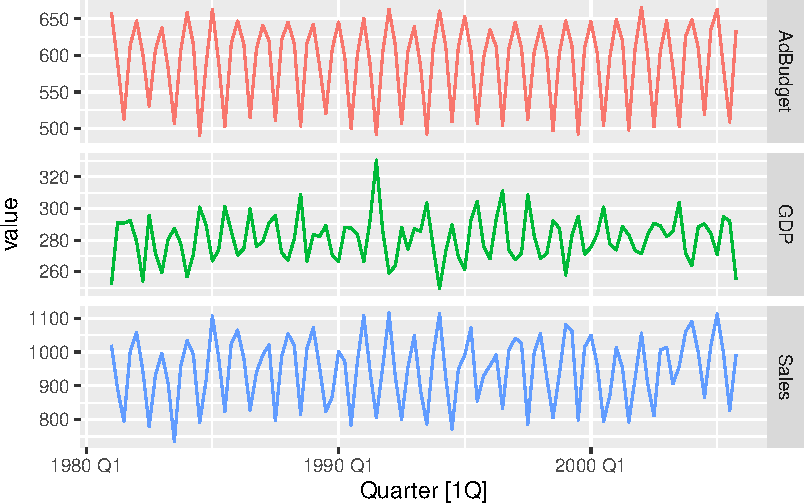
\includegraphics{index_files/figure-pdf/fig-deaths-1.pdf}

}

\caption{\label{fig-deaths}Quarterly sales, advertising and GDP data.}

\end{figure}

\hypertarget{results-from-analyses}{%
\section{Results from analyses}\label{results-from-analyses}}

We can fit a dynamic regression model to the sales data.

\begin{verbatim}
Series: Sales 
Model: LM w/ ARIMA(1,0,0)(0,1,1)[4] errors 

Coefficients:
         ar1     sma1     GDP  AdBudget
      0.2189  -0.9016  0.9742    2.2824
s.e.  0.1022   0.0715  0.4387    0.3930

sigma^2 estimated as 1677:  log likelihood=-493.94
AIC=997.87   AICc=998.54   BIC=1010.69
\end{verbatim}

If \(y_t\) denotes the sales in quarter \(t\), \(x_t\) denotes the
corresponding advertising budget and \(z_t\) denotes the GDP, then the
resulting model is: \begin{equation}\protect\hypertarget{eq-drm}{}{
  y_t - y_{t-4} = \beta (x_t-x_{t-4}) + \gamma (z_t-z_{t-4}) + \phi_1 (y_{t-1} - y_{t-5}) + \Theta_1 \varepsilon_{t-4} + \varepsilon_t
}\label{eq-drm}\end{equation} where \(\beta = 2.28\), \(\gamma = 0.97\),
\(\phi_1 = 0.22\), and \(\Theta_1 = -0.90\). We can reference this
equation using Equation~\ref{eq-drm}.

\hypertarget{tables}{%
\section{Tables}\label{tables}}

Let's assume future advertising spend and GDP are at the current levels.
Then forecasts for the next year are given in
Table~\ref{tbl-salesforecasts}.

\hypertarget{tbl-salesforecasts}{}
\begin{longtable}[]{@{}lr@{}}
\caption{\label{tbl-salesforecasts}Forecasts for the next year assuming
Advertising budget and GDP are unchanged.}\tabularnewline
\toprule\noalign{}
Quarter & Sales forecast \\
\midrule\noalign{}
\endfirsthead
\toprule\noalign{}
Quarter & Sales forecast \\
\midrule\noalign{}
\endhead
\bottomrule\noalign{}
\endlastfoot
2006 Q1 & 1000.2 \\
2006 Q2 & 1013.1 \\
2006 Q3 & 1076.7 \\
2006 Q4 & 1003.5 \\
\end{longtable}

Again, notice the use of labels and references to automatically generate
table numbers.

\bookmarksetup{startatroot}

\hypertarget{sec-style}{%
\chapter{This is a chapter-level heading}\label{sec-style}}

\hypertarget{this-is-the-first-section-level-heading}{%
\section{This is the first section-level
heading}\label{this-is-the-first-section-level-heading}}

Nam dui ligula, fringilla a, euismod sodales, sollicitudin vel, wisi.
Morbi auctor lorem non justo. Nam lacus libero, pretium at, lobortis
vitae, ultricies et, tellus. Donec aliquet, tortor sed accumsan
bibendum, erat ligula aliquet magna, vitae ornare odio metus a mi. Morbi
ac orci et nisl hendrerit mollis. Suspendisse ut massa. Cras nec ante.
Pellentesque a nulla. Cum sociis natoque penatibus et magnis dis
parturient montes, nascetur ridiculus mus. Aliquam tincidunt urna. Nulla
ullamcorper vestibulum turpis. Pellentesque cursus luctus mauris.

\begin{quote}
Nulla malesuada porttitor diam. Donec felis erat, congue non, volutpat
at, tincidunt tristique, libero. Vivamus viverra fermentum felis. Donec
nonummy pellentesque ante. Phasellus adipiscing semper elit. Proin
fermentum massa ac quam. Sed diam turpis, molestie vitae, placerat a,
molestie nec, leo. Maecenas lacinia. Nam ipsum ligula, eleifend at,
accumsan nec, suscipit a, ipsum. Morbi blandit ligula feugiat magna.
Nunc eleifend consequat lorem. Sed lacinia nulla vitae enim.
Pellentesque tincidunt purus vel magna. Integer non enim. Praesent
euismod nunc eu purus. Donec bibendum quam in tellus. Nullam cursus
pulvinar lectus. Donec et mi. Nam vulputate metus eu enim. Vestibulum
pellentesque felis eu massa.
\end{quote}

Quisque ullamcorper placerat ipsum. Cras nibh. Morbi vel justo vitae
lacus tincidunt ultrices. Lorem ipsum dolor sit amet, consectetuer
adipiscing elit. In hac habitasse platea dictumst. Integer tempus
convallis augue. Etiam facilisis. Nunc elementum fermentum wisi. Aenean
placerat. Ut imperdiet, enim sed gravida sollicitudin, felis odio
placerat quam, ac pulvinar elit purus eget enim. Nunc vitae tortor.
Proin tempus nibh sit amet nisl. Vivamus quis tortor vitae risus porta
vehicula.

\hypertarget{this-is-the-first-sub-section-level-heading}{%
\subsection{This is the first sub-section-level
heading}\label{this-is-the-first-sub-section-level-heading}}

Nam dui ligula, fringilla a, euismod sodales, sollicitudin vel, wisi.
Morbi auctor lorem non justo. Nam lacus libero, pretium at, lobortis
vitae, ultricies et, tellus. Donec aliquet, tortor sed accumsan
bibendum, erat ligula aliquet magna, vitae ornare odio metus a mi. Morbi
ac orci et nisl hendrerit mollis. Suspendisse ut massa. Cras nec ante.
Pellentesque a nulla. Cum sociis natoque penatibus et magnis dis
parturient montes, nascetur ridiculus mus. Aliquam tincidunt urna. Nulla
ullamcorper vestibulum turpis. Pellentesque cursus luctus mauris.

\begin{quote}
Nulla malesuada porttitor diam. Donec felis erat, congue non, volutpat
at, tincidunt tristique, libero. Vivamus viverra fermentum felis. Donec
nonummy pellentesque ante. Phasellus adipiscing semper elit. Proin
fermentum massa ac quam. Sed diam turpis, molestie vitae, placerat a,
molestie nec, leo. Maecenas lacinia. Nam ipsum ligula, eleifend at,
accumsan nec, suscipit a, ipsum. Morbi blandit ligula feugiat magna.
Nunc eleifend consequat lorem. Sed lacinia nulla vitae enim.
Pellentesque tincidunt purus vel magna. Integer non enim. Praesent
euismod nunc eu purus. Donec bibendum quam in tellus. Nullam cursus
pulvinar lectus. Donec et mi. Nam vulputate metus eu enim. Vestibulum
pellentesque felis eu massa.
\end{quote}

Quisque ullamcorper placerat ipsum. Cras nibh. Morbi vel justo vitae
lacus tincidunt ultrices. Lorem ipsum dolor sit amet, consectetuer
adipiscing elit. In hac habitasse platea dictumst. Integer tempus
convallis augue. Etiam facilisis. Nunc elementum fermentum wisi. Aenean
placerat. Ut imperdiet, enim sed gravida sollicitudin, felis odio
placerat quam, ac pulvinar elit purus eget enim. Nunc vitae tortor.
Proin tempus nibh sit amet nisl. Vivamus quis tortor vitae risus porta
vehicula.

\hypertarget{this-is-the-first-sub-sub-section-level-heading}{%
\subsubsection{This is the first sub-sub-section-level
heading}\label{this-is-the-first-sub-sub-section-level-heading}}

\hypertarget{this-is-the-first-paragraph-level-heading}{%
\paragraph{This is the first paragraph-level
heading}\label{this-is-the-first-paragraph-level-heading}}

\hypertarget{this-is-the-first-sub-paragraph-level-heading}{%
\subparagraph{This is the first sub-paragraph-level
heading}\label{this-is-the-first-sub-paragraph-level-heading}}

\hypertarget{citation-examples}{%
\section{Citation examples}\label{citation-examples}}

The contents of this section differ depending on the bibliography
settings, specifically whether the `usebiblatex' toggle is set to `true'
or `false'. This sentence shows citation with natbib (Pathak et al.
2007). This is another sentence showing citation with natbib
(Searchinger et al. 2013).

\hypertarget{footnote-examples}{%
\section{Footnote examples}\label{footnote-examples}}

This is a sentence followed by a footnote.\footnote{Mauris ut leo. Cras
  viverra metus rhoncus sem. Nulla et lectus vestibulum urna fringilla
  ultrices. Phasellus eu tellus sit amet tortor gravida placerat.
  Integer sapien est, iaculis in, pretium quis, viverra ac, nunc.
  Praesent eget sem vel leo ultrices biben- dum. Aenean faucibus. Morbi
  dolor nulla, malesuada eu, pulvinar at, mollis ac, nulla.} This is
another sentence followed by a footnote.\footnote{Mauris ut leo. Cras
  viverra metus rhoncus sem. Nulla et lectus vestibulum urna fringilla
  ultrices. Phasellus eu tellus sit amet tortor gravida placerat.
  Integer sapien est, iaculis in, pretium quis, viverra ac, nunc.
  Praesent eget sem vel leo ultrices biben- dum. Aenean faucibus. Morbi
  dolor nulla, malesuada eu, pulvinar at, mollis ac, nulla.}

\hypertarget{block-quote-example}{%
\section{Block quote example}\label{block-quote-example}}

The following is a block quote:

\hypertarget{endnote-examples}{%
\section{Endnote examples}\label{endnote-examples}}

Endnotes appear in a separate section after chapters and before the
reference list. This is a sentence followed by a endnote. This is
another sentence followed by a endnote. And here is a really long
endnote to show formatting across several pages.

\hypertarget{table-example}{%
\section{Table example}\label{table-example}}

See Table~\ref{tbl-table1} for an example of a table. Citing another
reference in caption is also straightforward. See Table~\ref{tbl-table2}
for a demonstration.

\hypertarget{tbl-table1}{}
\begin{longtable}[]{@{}lll@{}}
\caption{\label{tbl-table1}Here is a table caption that is especially
long to show what happens when it extends to more than one line in the
table of contents}\tabularnewline
\toprule\noalign{}
Column1 & Column2 & Column3 \\
\midrule\noalign{}
\endfirsthead
\toprule\noalign{}
Column1 & Column2 & Column3 \\
\midrule\noalign{}
\endhead
\bottomrule\noalign{}
\endlastfoot
Row1 & 1.0 & 2.0 \\
Row2 & 2.0 & 4.0 \\
Row1 & 3.0 & 6.0 \\
\end{longtable}

\hypertarget{tbl-table2}{}
\begin{longtable}[]{@{}lll@{}}
\caption{\label{tbl-table2}This table caption refers to another caption:
see Figure~\ref{fig-figexample}.}\tabularnewline
\toprule\noalign{}
Column1 & Column2 & Column3 \\
\midrule\noalign{}
\endfirsthead
\toprule\noalign{}
Column1 & Column2 & Column3 \\
\midrule\noalign{}
\endhead
\bottomrule\noalign{}
\endlastfoot
Row1 & 1.0 & 2.0 \\
Row2 & 2.0 & 4.0 \\
Row1 & 3.0 & 6.0 \\
\end{longtable}

\begin{longtable}[]{@{}lll@{}}
\caption{This table caption refers to another caption: see
Figure~\ref{fig-figexample}.}\tabularnewline
\toprule\noalign{}
Column1 & Column2 & Column3 \\
\midrule\noalign{}
\endfirsthead
\toprule\noalign{}
Column1 & Column2 & Column3 \\
\midrule\noalign{}
\endhead
\bottomrule\noalign{}
\endlastfoot
Row1 & 1.0 & 2.0 \\
Row2 & 2.0 & 4.0 \\
Row1 & 3.0 & 6.0 \\
\end{longtable}

\hypertarget{figure-example}{%
\section{Figure example}\label{figure-example}}

See Figure~\ref{fig-figexample} for an example of a figure.

\begin{figure}

{\centering 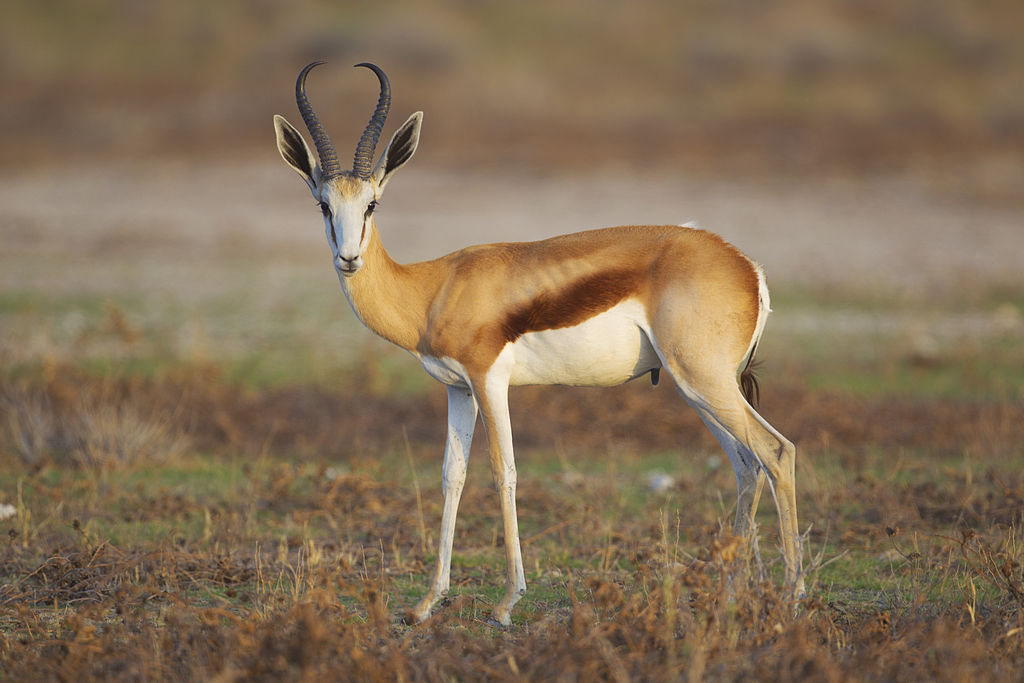
\includegraphics{chapters/../img/antidorcas.png}

}

\caption{\label{fig-figexample}Antidorcas marsupialis, male}

\end{figure}

\hypertarget{math-examples}{%
\section{Math examples}\label{math-examples}}

This section contains some math-heavy text adapted from Wilkins (1995).
In non-relativistic wave mechanics, the wave function
\(\psi(\mathbf{r},t)\) of a particle satisfies the Schrödinger Wave
Equation \[i\hbar\frac{\partial \psi}{\partial t}
    = \frac{-\hbar^2}{2m} \left(
    \frac{\partial^2}{\partial x^2}
    + \frac{\partial^2}{\partial y^2}
    + \frac{\partial^2}{\partial z^2}
    \right) \psi + V \psi.\] It is customary to normalize the wave
equation by demanding that \[\int \!\!\! \int \!\!\! \int_{\textbf{R}^3}
    \left| \psi(\mathbf{r},0) \right|^2\,dx\,dy\,dz = 1.\] A simple
calculation using the Schrödinger wave equation shows that
\[\frac{d}{dt} \int \!\!\! \int \!\!\! \int_{\textbf{R}^3}
    \left| \psi(\mathbf{r},t) \right|^2\,dx\,dy\,dz = 0,\] and hence
\[\int \!\!\! \int \!\!\! \int_{\textbf{R}^3}
    \left| \psi(\mathbf{r},t) \right|^2\,dx\,dy\,dz = 1\] for all
times~\(t\). If we normalize the wave function in this way then, for any
(measurable) subset~\(V\) of \(\textbf{R}^3\) and time~\(t\),
\[\int \!\!\! \int \!\!\! \int_V
    \left| \psi(\mathbf{r},t) \right|^2\,dx\,dy\,dz\] represents the
probability that the particle is to be found within the region~\(V\) at
time~\(t\).

\bookmarksetup{startatroot}

\hypertarget{references}{%
\chapter*{REFERENCES}\label{references}}
\addcontentsline{toc}{chapter}{REFERENCES}

\markboth{REFERENCES}{REFERENCES}

\hypertarget{refs}{}
\begin{CSLReferences}{1}{0}
\leavevmode\vadjust pre{\hypertarget{ref-pathak_rural_2007}{}}%
Pathak, P, SP Wani, R Sudi, AK Chourasia, SN Singh, and Kesava Rao.
2007. \emph{Rural Prosperity Through Integrated Watershed Management: A
Case Study of Gokulpura--Goverdhanpura in Eastern Rajasthan}. Global
Theme on Agroecosystems 36. Patancheru, India: International Crops
Research Institute for the Semi-Arid Tropics ({ICRISAT}).
\url{http://www.icrisat.org/Journal/volume5/aes/aes6.pdf}.

\leavevmode\vadjust pre{\hypertarget{ref-searchinger_world_2013}{}}%
Searchinger, Tim, Craig Hanson, Janet Ranganathan, Brian Lipinski,
Richard Waite, Robert Winterbottom, Ayesha Dinshaw, and Ralph Heimlich.
2013. \emph{World Resources Report 2013--14: Interim Findings---Creating
a Sustainable Food Future}. Washington, {DC}: World Resources Institute.
\url{http://www.wri.org/sites/default/files/WRI13_Report_4c_WRR_online.pdf}.

\leavevmode\vadjust pre{\hypertarget{ref-dwilkins1995}{}}%
Wilkins, David R. 1995. \emph{Getting Started with LaTeX}. 2nd ed.
\url{http://www.maths.tcd.ie/~dwilkins/LaTeXPrimer/}.

\end{CSLReferences}

\cleardoublepage
\phantomsection
\addcontentsline{toc}{part}{Appendices}
\appendix

\hypertarget{additional-stuff}{%
\chapter{Additional stuff}\label{additional-stuff}}

You might put some computer output here, or maybe additional tables. It
is possible to have multiple appendices. Just list them in the
appropriate place within \texttt{\_quarto.yml}.

%%%%%%%%%%%%%%%%%%%%%%%%%%%%%%%%%%%%%%%
% Back matter
%%%%%%%%%%%%%%%%%%%%%%%%%%%%%%%%%%%%%%%
\SingleSpacing                          % Back matter should be single spaced
\AfterEndEnvironment{table}{\SingleSpacing} % Reset these environments
\AfterEndEnvironment{figure}{\SingleSpacing}
\AfterEndEnvironment{quote}{\SingleSpacing}
\AfterEndEnvironment{quotation}{\SingleSpacing}

\edef\defaulttolerance{\the\tolerance}
\tolerance 500                          % Increase tolerance to prevent material extending into margins
\hbadness 500

\iftoggle{useendnotes}{%                % If you're using endnotes, output them here
	\setsecnumdepth{none}                 % No section numbering in end notes
	\bookmarksetup{startatroot}           % Make Notes appear at root level of PDF bookmarks
	\phantomsection%                      % Need for hyperref
	\addcontentsline{toc}{chapter}{%      % Add a chapter-level heading for
		\hspace{-\cftchapterindent}%        %  Notes to the ToC
		\notesname%
	}%
	\renewcommand*{\notedivision}{%
		\chapter*{\notesname}%
	}
	\printpagenotes                       % Output the notes
	\setsecnumdepth{all}%                 % Turn section numbering back on after printing
}{}

\bookmarksetup{startatroot}
\chapter*{\bibheading}                  % In the running text, use a chapter-level heading
% for the bibliography section
\phantomsection
\addcontentsline{toc}{chapter}{%        % In the TOC, add a custom chapter-level heading
	\hspace{-\cftchapterindent}%          % that will be flush against the left margin
	\bibheading%
}
%\phantomsection
%\addtocontents{toc}%                    % Add this 'mark' to TOC so subsequent pages use
%  {\protect\markboth{\bibheading}{Page}}%   the bibliography heading (unlikely since
%                                        %   the appendices follow quickly)
\iftoggle{usebiblatex}{%                % Output the bibliography
	\printbibliography[heading=none]      % Using a 'biblatex' package; do not let
	%   'biblatex' output a heading
}{%
	\renewcommand\bibsection{}            % Do not let 'natbib' output a heading
	\bibliographystyle{\natbibstyle}      % Using 'natbib' to print bibliography
	\bibliography{\bibfilename}
}

\appendix                               % Indicate start of appendices
% Appendices are considered 'mainmatter' in this
%   documentclass
\tolerance \defaulttolerance            % Set tolerance back to default
\hbadness \defaulttolerance

\addtocontents{toc}{\protect%           % Only include appendix title in table of contents
	\setcounter{tocdepth}{0}}%            %   and omit sub-headings
\renewcommand*{\chapnamefont}%          % Reset font for 'Appendix' in chapter titles
{\normalfont\MakeTextUppercase}
\makeatletter                           % Clear page after printing appendix title
\renewcommand{\memendofchapterhook}%
{%
	\clearpage
	\m@mindentafterchapter
	\@afterheading
}
\makeatother

\phantomsection                         % Need '\phantomsection' to place hyperref
%   bookmark more accurately
\addcontentsline{toc}{part}{Appendix}   %~Add "Appendix" to TOC here; comment out this
%   line if you're not including appendices

%\phantomsection                        %!This is the one part of the template that I
%\addtocontents{toc}%                   %   could not get to work properly. After you
%  {\protect\markboth{APPENDIX}{Page}}  %   start listing appendices in the TOC,
%   subsequent TOC pages should use "APPENDIX in
%   the header instead of "CHAPTER"; however,
%   this code will make "APPENDIX" appear on the
%   the same page that the *first* appendix
%   appears on. This problem won't affect most
%   people, but if it affects you, uncomment
%   these lines and move them below where
%   the appendices are listed. Keep moving these
%   lines down and checking the output until
%   the TOC headers appear correctly

%\input{appendix1}                       %~Insert your appendices here; I recommend to use
%\input{appendix2}                       %   \input rather than \include for appendices.
%\input{appendix3}% etc.                 %   All heading commands are the same as above,
%   e.g., \chapter, \section, etc.


\backmatter                             % Start back matter according to documentclass
\makeatletter                           % Do not clear page after printing title for
\renewcommand{\memendofchapterhook}%  %   biographical sketch
{%
	\m@mindentafterchapter
	\@afterheading
}
\makeatother

\biographicalsketch{% Your biosketch written in LaTex

Lorem ipsum dolor sit amet, consectetuer adipiscing elit. Ut purus elit, vestibulum ut,
placerat ac, adipiscing vitae, felis. Curabitur dictum gravida mauris. Nam arcu libero,
nonummy eget, consectetuer id, vulputate a, magna. Donec vehicula augue eu neque.
Pellentesque habitant morbi tristique senectus et netus et malesuada fames ac turpis
egestas. Mauris ut leo. Cras viverra metus rhoncus sem. Nulla et lectus vestibulum urna
fringilla ultrices. Phasellus eu tellus sit amet tortor gravida placerat. Integer sapien
est, iaculis in, pretium quis, viverra ac, nunc.
}

\end{document}
